\newpage
\section{Part C/D}
\label{sec:sec_cd}

A naive algorithm was applied to the data set, in which a random value for \textit{b} and \textit{w} is chosen. For each  pair the MSE is computed, if it is lower than the previous best pair, the pair is saved and the best MSE is updated. This algorithm was let to run for 1000 iterations. Upon completion the best pair tested was $b=0.0314$ and $w=1.035$ which gave an MSE of $0.05487$. In comparison to the "golden" values found in Section~\ref{sec:sec_a} it can be seen that the algorithm was able to produce similar values.

The loss surface is again plotted, marking the \textit{b} and \textit{w} pairs which improved the MSE it can be seen then each improvement is closer to the "golden" value. However due to the random nature of the algorithm the iterations do not travel along any predictable path.

\begin{figure}[htpb]
	\centering
	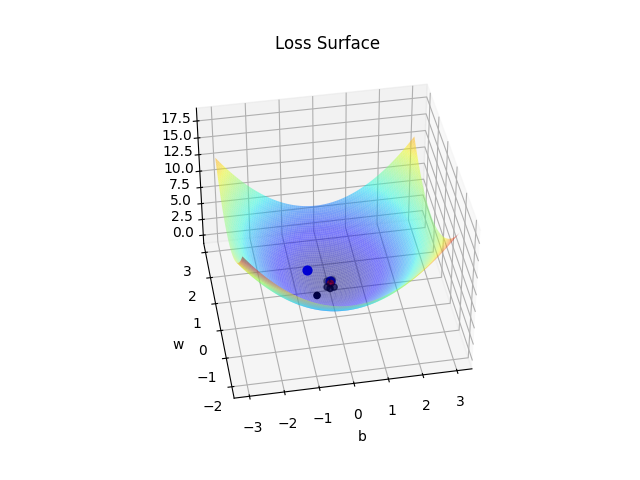
\includegraphics[width=\columnwidth]{figures/loss_surface_naive.png}
	\label{fig:loss_surface_naive}
\end{figure}

\LST{part\_c}